\section{Технический проект}
\subsection{Общая характеристика архитектуры решения}

Графический движок представляет собой кроссплатформенное приложение для визуализации трёхмерных сцен, построенное на следующих ключевых компонентах:

\begin{itemize}
    \item подсистема управления окнами (SDL2);
    \item графический конвейер (OpenGL 3.3);
    \item подсистема загрузки ресурсов (текстуры, шейдеры);
    \item менеджер сцен и объектов.
\end{itemize}

Движок спроектирован как модульная система, позволяющая расширять функционал без изменения ядра.

\subsection{Обоснование выбора технологий}

\subsubsection{Язык программирования C++}

В качестве основного языка разработки выбран C++ -- высокопроизводительный компилируемый язык, обеспечивающий прямой доступ к API библиотек. Его кроссплатформенная природа позволяет компилировать движок под различные операционные системы без изменения исходного кода. Современные стандарты C++ предоставляют необходимые средства для эффективной работы с памятью и многопоточностью, что критично для графических приложений.

\subsubsection{Система сборки CMake}

В качестве системы управления сборкой в проекте применяется CMake, что обусловлено его гибкостью и широкой поддержкой в индустрии разработки программного обеспечения. Использование CMake позволяет централизованно описывать структуру проекта, автоматически находить и подключать сторонние библиотеки, а также формировать корректные проекты для различных платформ и сред разработки. Современные стандарты CMake делают сборочный процесс прозрачным и легко масштабируемым: добавление новых исходных файлов или зависимостей не требует ручных изменений для каждой платформы.

Использование подобной системы минимизирует вероятность ошибок, связанных с различиями между платформами, и ускоряет процесс разработки.

\subsubsection{Компилятор GCC}

Для компиляции движка был выбран бесплатный компилятор с открытым исходным кодом GCC (GNU Compiler Collection), обеспечивающий возможность компиляции C и C++ кода с поддержкой современных стандартов. GCC по-умолчанию поддерживается только на операционной системе Linux, но имеет возможность компиляции под Windows с помощью MinGW.

\subsubsection{Набор инструментов разработки MinGW}

Для сборки и запуска проекта на платформе Windows используется набор инструментов разработки MinGW (Minimalist GNU for Windows), который предоставляет среду для работы с GCC. Он также обеспечивает совместимость с другими инструментами Linux, что облегчает переносимость кода между платформами, а также позволяют использовать единые скрипты сборки и тестирования.

В процессе разработки данного проекта MinGW показал себя как надёжное и удобное решение для удобной разработки под Windows.

\subsubsection{Библиотека SDL2}

Для взаимодействия с оконной системой используется библиотека SDL2 (Simple DirectMedia Layer), которая абстрагирует платформозависимые особенности создания окон, обработки ввода и работы с аудио. SDL2 была выбрана благодаря своей стабильности, поддержке нескольких платформ и минимальным затратам времени на адаптацию. Библиотека предоставляет простой API для инициализации графического контекста OpenGL и обработки пользовательского ввода.

\subsubsection{Спецификация графического API OpenGL}

Графический конвейер реализован на основе OpenGL 3.3 Core Profile -- кроссплатформенного графического API, поддерживаемого большинством современных видеокарт. Выбор версии 3.3 обусловлен балансом между функциональностью и совместимостью: этот стандарт предоставляет современный конвейер рендеринга с шейдерной моделью, но при этом не требует новейшей аппаратуры.

Для привязки аппаратных функций OpenGL к структурам языка C++ используется загрузочная библиотека Glad.

OpenGL был предпочтен Vulkan и Direct3D ввиду своей универсальности и меньшего порога входа.

\subsubsection{Язык программирования шейдеров GLSL}

GLSL (OpenGL Shading Language) является языком программирования для написания шейдеров, используемых в конвейере рендеринга. Шейдеры позволяют конечным пользователям настраивать различные аспекты визуализации, такие как текстуры, освещение и эффекты, без перекомпиляции основной части программы. Все операции шейдеров выполняются на графическом ускорителе, что обеспечивает высокую производительность.

\subsubsection{Математическая библиотека GLM}

Библиотека GLM (OpenGL Mathematics) предоставляет математические функции и типы данных, специфичные для компьютерной графики:

\begin{itemize}
    \item операции с векторами и матрицами (произведение, сложение, вычитание);
    \item трансформации (перемещение, вращение, масштабирование);
    \item пространственных преобразований (нормализация, проекции).
\end{itemize}

GLM применяется в движке для упрощения таких действий, как расчёт матриц модели, вида и проекции, преобразование координат и управление камерой и перспективой.

Библиотека была выбрана благодаря полной совместимости с OpenGL, оптимизированным SIMD-операциям и удобному синтаксису, аналогичному GLSL.

\subsection{Архитектурные компоненты системы}

Диаграмма компонентов (рис. \ref{comp:image}) отражает физическую и логическую структуру графического движка. Архитектура системы построена по принципу разделения ответственности, где каждый компонент инкапсулирует строго определённую функциональность.

\afterpage{
  \begin{landscape}
    \begin{figure}[p]
      \centering
      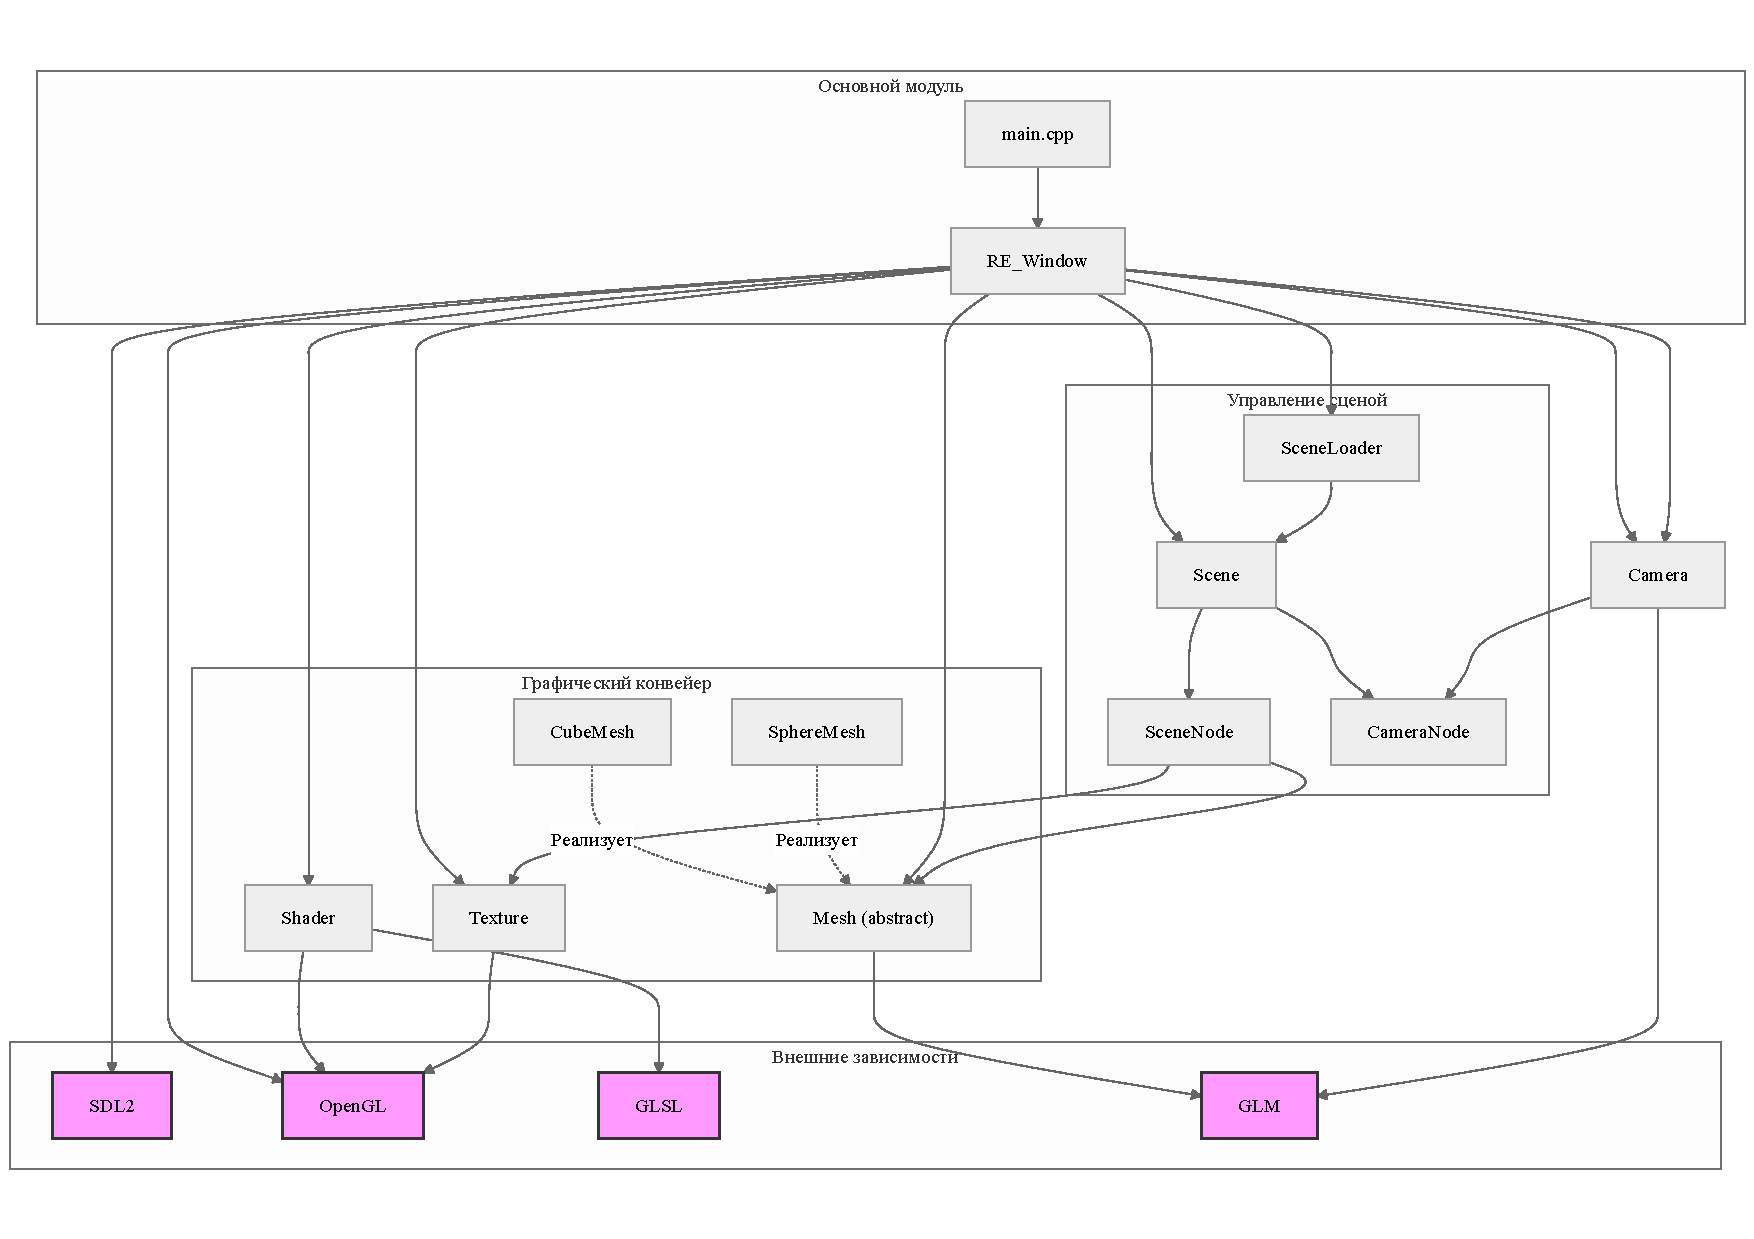
\includegraphics[width=1.3\textwidth]{comp.pdf}
      \caption{Диаграмма компонентов движка с последовательностью взаимодействия}
      \label{comp:image}
    \end{figure}
  \end{landscape}
}


\subsubsection{Состав компонентов}

Основные модули системы включают:

\begin{enumerate}
    \item RE\_Window -- компонент управления оконным контекстом, реализующий абстракцию над библиотекой SDL2. Обеспечивает:

    \begin{itemize}[itemindent=\parindent,leftmargin=\parindent]
        \item создание и настройку графического окна;
        \item инициализацию контекста OpenGL;
        \item обработку системных событий и пользовательского ввода.
    \end{itemize}

    \item Scene и SceneLoader -- подсистема работы со сценой:

    \begin{itemize}[itemindent=\parindent,leftmargin=\parindent]
        \item SceneLoader загружает список объектов из .rem-файлов;
        \item Scene хранит коллекцию объектов (SceneNode) и управляет их состоянием.
    \end{itemize}

    \item Графический конвейер (неявный компонент):

    \begin{itemize}[itemindent=\parindent,leftmargin=\parindent]
        \item Shader -- управление шейдерными программами (вершинный/фрагментный);
        \item Texture -- загрузка, генерация и привязка текстурных объектов;
        \item Mesh/СubeMesh/SphereMesh -- хранение геометрических данных (VBO/VAO/EBO).
    \end{itemize}

    \item Camera -- компонент управления видами, реализующий:

    \begin{itemize}[itemindent=\parindent,leftmargin=\parindent]
        \item расчёт матриц вида и проекции;
        \item преобразование координат;
        \item управление параметрами отображения.
    \end{itemize}
\end{enumerate}

\subsubsection{Взаимодействие компонентов}

Последовательность работы системы (рис. \ref{comp:image}) реализуется следующим образом:

\begin{enumerate}
    \item Инициализация:

    \begin{itemize}[itemindent=\parindent,leftmargin=\parindent]
        \item RE\_Window создаёт графический контекст;
        \item Shader компилирует шейдерные программы;
        \item SceneLoader загружает начальную сцену.
    \end{itemize}

    \item Главный цикл рендеринга:

    \begin{itemize}[itemindent=\parindent,leftmargin=\parindent]
        \item обновление матриц вида в Camera;
        \item передача uniform-переменных в шейдеры;
        \item формирование вершинного буфера объектов сцены из вектора SceneNode;
        \item отрисовка объектов сцены с учётом их:

        \begin{itemize}[itemindent=\parindent,leftmargin=\parindent]
            \item геометрии (Mesh);
            \item текстуры (Texture);
            \item шейдеров (Shader).
        \end{itemize}

        \item вывод результата через RE\_Window;
        \item обработка пользовательского ввода RE\_Window и передача его значений в Camera;
        \item повтор цикла до выхода из программы.
    \end{itemize}
\end{enumerate}

\subsection{Основные сущности системы}

Программная система состоит из сущностей, выраженных классами и структурами языка C++. Их взаимодействие реализуется через встроенные механизмы наследования и представлено в диаграмме UML (рис. \ref{uml:image}).

\afterpage{
  \begin{landscape}
    \begin{figure}[p]
      \centering
      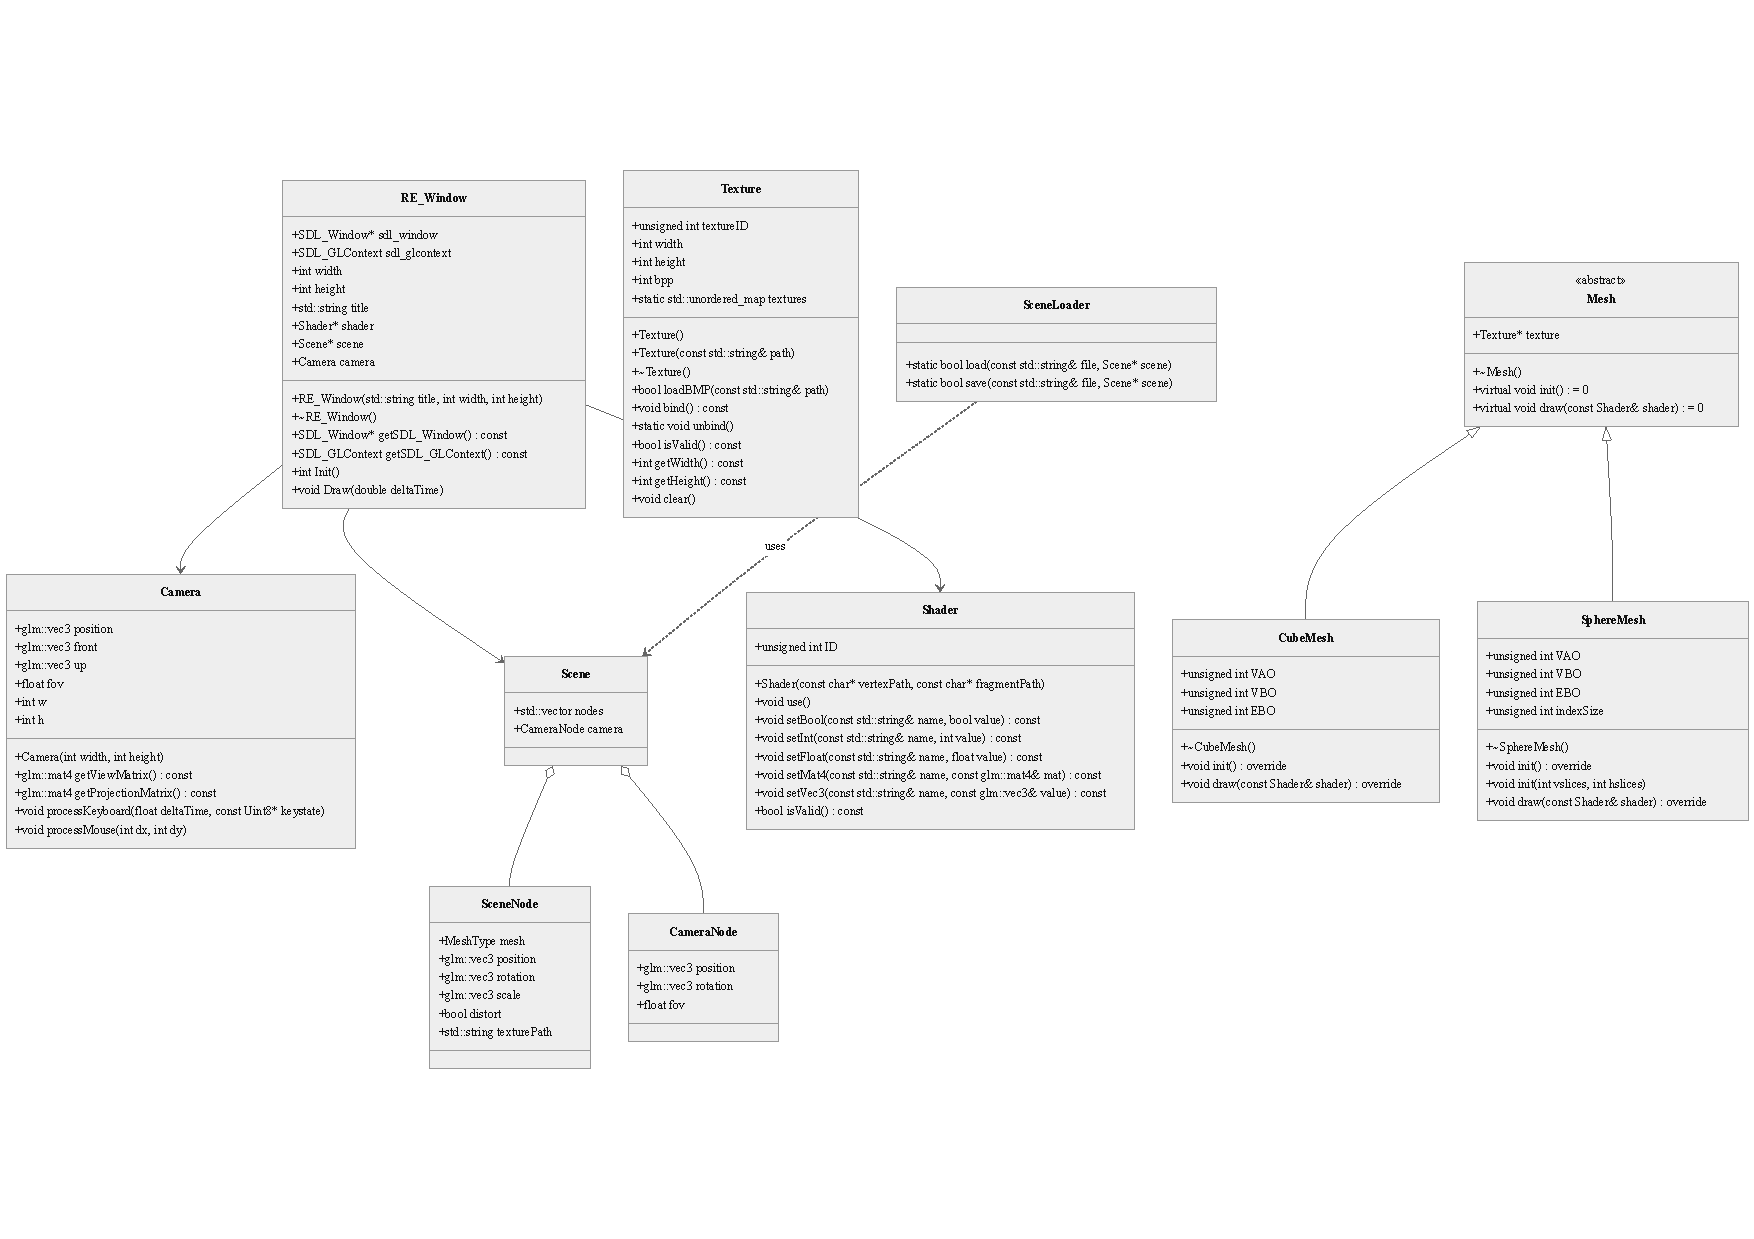
\includegraphics[width=1.3\textwidth]{uml.pdf}
      \caption{Диаграмма UML}
      \label{uml:image}
    \end{figure}
  \end{landscape}
}

\subsubsection{Класс RE\_Window}
Класс RE\_Window отвечает за создание и управление окном приложения, инициализацию и управление контекстом OpenGL, а также за отрисовку сцены. Он инкапсулирует низкоуровневые операции взаимодействия с библиотекой SDL2 для управления окном и событиями, предоставляя высокоуровневый интерфейс для основной логики приложения. Класс также содержит указатели на используемый шейдер, отображаемую сцену и камеру, через которую происходит просмотр.

Спецификация класса RE\_Window представлена в таблице \ref{tab:re_window_spec}.

\begin{xltabular}{\textwidth}{|X|l|X|}
    \caption{Спецификация класса RE\_Window\label{tab:re_window_spec}}\\ \hline
    \centrow Поле/Метод & \centrow Тип & \centrow Описание \\ \hline
    \endfirsthead
    \continuecaption{Продолжение таблицы \ref{tab:re_window_spec}}
    \centrow Поле/Метод & \centrow Тип & \centrow Описание \\ \hline 
    \finishhead

    \multicolumn{3}{|l|}{Поля} \\ \hline
    sdl\_window & SDL\_Window* & Указатель на структуру окна SDL2. Используется для непосредственного взаимодействия с оконной системой. \\
    \hline
    sdl\_glcontext & SDL\_GLContext & Контекст OpenGL, связанный с окном. Необходим для выполнения команд OpenGL. \\
    \hline
    width & int & Ширина окна в пикселях. \\
    \hline
    height & int & Высота окна в пикселях. \\
    \hline
    title & std::string & Заголовок окна, отображаемый в операционной системе. \\
    \hline
    shader & Shader* & Указатель на объект шейдера, используемый для рендеринга объектов сцены. \\
    \hline
    scene & Scene* & Указатель на объект сцены, содержащий все объекты для отображения. \\
    \hline
    camera & Camera & Объект камеры, определяющий точку обзора и параметры проекции. \\
    \hline
    \multicolumn{3}{|l|}{Методы} \\ \hline
    RE\_Window(std::string title, int width, int height) & конструктор & Конструктор класса. Инициализирует поля title, width и height. \\
    \hline
    \textasciitilde RE\_Window() & деструктор & Деструктор класса. Освобождает ресурсы, связанные с окном SDL2 и контекстом OpenGL. \\
    \hline
    getSDL\_Window() & SDL\_Window* & Возвращает указатель на окно SDL2. \\
    \hline
    getSDL\_GLContext() & SDL\_GLContext & Возвращает контекст OpenGL. \\
    \hline
    Init() & int & Инициализирует окно SDL2 и контекст OpenGL. Создает окно с заданными параметрами и настраивает OpenGL для рендеринга. Возвращает 0 при успехе. \\
    \hline
    Draw(double deltaTime) & void & Выполняет отрисовку одного кадра. Очищает буферы, устанавливает параметры рендеринга и вызывает методы отрисовки для объектов сцены. deltaTime — время, прошедшее с предыдущего кадра. \\
    \hline
\end{xltabular}

\subsubsection{Класс Texture}
Класс Texture предназначен для загрузки, хранения и управления текстурными данными, которые используются для наложения изображений на поверхности 3D-объектов. В текущей реализации поддерживается загрузка текстур из файлов формата BMP. Класс инкапсулирует взаимодействие с OpenGL для создания и управления текстурными объектами, а также предоставляет статический кеш для загруженных текстур, чтобы избежать повторной загрузки одних и тех же файлов.

Спецификация класса Texture представлена в таблице \ref{tab:texture_spec}.

\begin{xltabular}{\textwidth}{|X|X|X|}
    \caption{Спецификация класса Texture\label{tab:texture_spec}}\\ \hline
    \centrow Поле/Метод & \centrow Тип & \centrow Описание \\ \hline
    \endfirsthead
    \continuecaption{Продолжение таблицы \ref{tab:texture_spec}}
    \centrow Поле/Метод & \centrow Тип & \centrow Описание \\ \hline 
    \finishhead

    \multicolumn{3}{|l|}{Поля} \\ \hline
    textureID & unsigned int & Идентификатор текстурного объекта OpenGL. Используется для привязки и управления текстурой в графическом конвейере. \\
    \hline
    width & int & Ширина загруженной текстуры в пикселях. \\
    \hline
    height & int & Высота загруженной текстуры в пикселях. \\
    \hline
    bpp & int & Количество битов на пиксель в загруженной текстуре. \\
    \hline
    textures & static std::unordered\_map <std::string, Texture*> & Статический ассоциативный массив (кеш) для хранения загруженных текстур. Ключом является путь к файлу текстуры. \\
    \hline
    \multicolumn{3}{|l|}{Методы} \\ \hline
    Texture() & конструктор & Конструктор по умолчанию. Инициализирует поля значениями по умолчанию. \\
    \hline
    Texture(const std::string\& path) & конструктор & Конструктор, загружающий текстуру из указанного файла BMP. \\
    \hline
    \textasciitilde Texture() & деструктор & Деструктор класса. Освобождает ресурсы, связанные с текстурным объектом OpenGL. \\
    \hline
    loadBMP(const std::string\& path) & bool & Загружает текстуру из файла BMP. Возвращает true при успешной загрузке. \\
    \hline
    bind() & void & Привязывает текстуру (делает ее активной) для использования в последующих операциях рендеринга. \\
    \hline
    unbind() & static void & Отвязывает текущую активную текстуру. \\
    \hline
    isValid() & bool & Проверяет, была ли текстура успешно загружена и инициализирована (textureID $\neq$ 0). \\
    \hline
    getWidth() & int & Возвращает ширину текстуры. \\
    \hline
    getHeight() & int & Возвращает высоту текстуры. \\
    \hline
    clear() & void & Приватный метод для очистки данных текстуры и освобождения ресурсов OpenGL. \\
    \hline
\end{xltabular}

\subsubsection{Класс Shader}
Класс Shader инкапсулирует логику работы с шейдерными программами в OpenGL. Он отвечает за загрузку исходного кода вершинного и фрагментного шейдеров из файлов, их компиляцию и последующую линковку в единую шейдерную программу. Кроме того, класс предоставляет удобные методы для активации шейдерной программы и установки значений uniform-переменных различных типов (bool, int, float, vec3, mat4), которые используются для передачи данных из основного приложения в шейдеры во время рендеринга.

Спецификация класса Shader представлена в таблице \ref{tab:shader_spec}.

\begin{xltabular}{\textwidth}{|X|l|X|}
    \caption{Спецификация класса Shader\label{tab:shader_spec}}\\ \hline
    \centrow Поле/Метод & \centrow Тип & \centrow Описание \\ \hline
    \endfirsthead
    \continuecaption{Продолжение таблицы \ref{tab:shader_spec}}
    \centrow Поле/Метод & \centrow Тип & \centrow Описание \\ \hline 
    \finishhead

    \multicolumn{3}{|l|}{Поля} \\ \hline
    ID & unsigned int & Идентификатор скомпилированной и слинкованной шейдерной программы OpenGL. \\
    \hline
    \multicolumn{3}{|l|}{Методы} \\ \hline
    Shader(const char* vertexPath, const char* fragmentPath) & конструктор & Конструктор класса. Загружает, компилирует и линкует вершинный и фрагментный шейдеры по указанным путям к файлам. Сохраняет идентификатор программы в поле ID. \\
    \hline
    use() & void & Активирует данную шейдерную программу для использования в последующих операциях рендеринга. \\
    \hline
    setBool(const std::string \&name, bool value) const & void & Устанавливает значение uniform-переменной типа bool в шейдере. \\
    \hline
    setInt(const std::string \&name, int value) const & void & Устанавливает значение uniform-переменной типа int в шейдере. \\
    \hline
    setFloat(const std::string \&name, float value) const & void & Устанавливает значение uniform-переменной типа float в шейдере. \\
    \hline
    setMat4(const std::string \&name, const glm::mat4 \&mat) const & void & Устанавливает значение uniform-переменной типа mat4 (матрица 4x4) в шейдере. \\
    \hline
    setVec3(const std::string \&name, const glm::vec3 \&value) const & void & Устанавливает значение uniform-переменной типа vec3 (3D вектор) в шейдере. \\
    \hline
    isValid() const & bool & Проверяет, была ли шейдерная программа успешно скомпилирована и слинкована (ID $\neq$ 0). \\
    \hline
    checkCompileErrors(unsigned int shader, std::string type) & void & Приватный метод для проверки ошибок компиляции или линковки шейдера/программы и вывода информации об ошибке. \\
    \hline
\end{xltabular}

\subsubsection{Класс Mesh}
Класс Mesh является абстрактным базовым классом, представляющим собой интерфейс для всех трехмерных геометрических объектов (примитивов), которые могут быть отрисованы в сцене. Он определяет основные операции, которые должен поддерживать каждый конкретный тип примитива: инициализацию геометрических данных (вершин, их атрибутов, индексов) и их последующую отрисовку с использованием заданной шейдерной программы. Класс также содержит указатель на объект Texture, что позволяет связывать текстуры с примитивами.

Поскольку класс Mesh абстрактный, его экземпляры не могут быть созданы напрямую. Вместо этого создаются экземпляры его производных классов, таких как CubeMesh или SphereMesh, которые реализуют его чисто виртуальные методы.

Спецификация класса Mesh представлена в таблице \ref{tab:mesh_spec}.

\begin{xltabular}{\textwidth}{|l|l|X|}
    \caption{Спецификация класса Mesh\label{tab:mesh_spec}}\\ \hline
    \centrow Поле/Метод & \centrow Тип & \centrow Описание \\ \hline
    \endfirsthead
    \continuecaption{Продолжение таблицы \ref{tab:mesh_spec}}
    \centrow Поле/Метод & \centrow Тип & \centrow Описание \\ \hline 
    \finishhead

    \multicolumn{3}{|l|}{Поля} \\ \hline
    texture & Texture* & Указатель на объект текстуры, который может быть применен к данному примитиву. Если nullptr, примитив будет отрисован без текстуры или с использованием цвета по умолчанию. \\
    \hline
    \multicolumn{3}{|l|}{Методы} \\ \hline
    \textasciitilde Mesh() & виртуальный деструктор & Виртуальный деструктор по умолчанию. Обеспечивает корректное освобождение ресурсов при удалении объектов производных классов через указатель на базовый класс. \\
    \hline
    init() & virtual void = 0 & Виртуальный метод для инициализации примитива. В производных классах здесь должна происходить загрузка вершинных данных в буферы OpenGL (VBO, VAO, EBO). \\
    \hline
    draw(const Shader\& shader) & virtual void = 0 & Виртуальный метод для отрисовки примитива. В производных классах здесь должны выполняться команды OpenGL для отрисовки геометрии с использованием переданного шейдера. \\
    \hline
\end{xltabular}

\subsubsection{Класс CubeMesh}
Класс CubeMesh является производным от абстрактного класса Mesh и предоставляет конкретную реализацию для создания и отрисовки трехмерного куба. Он отвечает за определение вершин, их атрибутов (например, позиций, текстурных координат, нормалей) и индексов, необходимых для формирования геометрии куба. В методе init() происходит создание и настройка буферных объектов OpenGL (VAO, VBO, EBO) для хранения этих данных. Метод draw() использует эти буферы для выполнения команд отрисовки куба с помощью предоставленного шейдера.

Спецификация класса CubeMesh представлена в таблице \ref{tab:cubemesh_spec}.

\begin{xltabular}{\textwidth}{|l|l|X|}
    \caption{Спецификация класса CubeMesh\label{tab:cubemesh_spec}}\\ \hline
    \centrow Поле/Метод & \centrow Тип & \centrow Описание \\ \hline
    \endfirsthead
    \continuecaption{Продолжение таблицы \ref{tab:cubemesh_spec}}
    \centrow Поле/Метод & \centrow Тип & \centrow Описание \\ \hline 
    \finishhead

    \multicolumn{3}{|l|}{Поля} \\ \hline
    VAO & unsigned int & Идентификатор объекта вершинного массива (Vertex Array Object). Хранит конфигурацию атрибутов вершин для куба. \\
    \hline
    VBO & unsigned int & Идентификатор объекта вершинного буфера (Vertex Buffer Object). Хранит данные о вершинах куба (координаты, текстурные координаты и т.д.). \\
    \hline
    EBO & unsigned int & Идентификатор объекта элементного буфера (Element Buffer Object) или индексного буфера. Хранит индексы вершин для формирования граней куба. \\
    \hline
    \multicolumn{3}{|l|}{Методы} \\ \hline
    \textasciitilde CubeMesh() & деструктор & Деструктор класса. Освобождает ресурсы OpenGL, выделенные для VAO, VBO и EBO. \\
    \hline
    init() & void override & Реализация виртуального метода базового класса. Инициализирует геометрию куба: определяет вершины и индексы, создает и заполняет буферы VAO, VBO, EBO. \\
    \hline
    draw(const Shader\& shader) & void override & Реализация виртуального метода базового класса. Выполняет отрисовку куба: привязывает VAO, активирует шейдер и вызывает команду отрисовки по индексам (glDrawElements). \\
    \hline
\end{xltabular}

\subsubsection{Класс SphereMesh}
Класс SphereMesh наследует от абстрактного класса Mesh и отвечает за создание и отрисовку трехмерной сферы. Он генерирует вершины, текстурные координаты и индексы, необходимые для аппроксимации сферической поверхности. Точность аппроксимации (количество полигонов) может контролироваться через параметры, передаваемые в один из его методов инициализации (количество вертикальных и горизонтальных сегментов). Как и куб, SphereMesh управляет собственными буферными объектами OpenGL (VAO, VBO, EBO) для хранения геометрии и её последующей отрисовки.

Спецификация класса SphereMesh представлена в таблице \ref{tab:spheremesh_spec}.
\begin{xltabular}{\textwidth}{|l|l|X|}
    \caption{Спецификация класса SphereMesh\label{tab:spheremesh_spec}}\\ \hline
    \centrow Поле/Метод & \centrow Тип & \centrow Описание \\ \hline
    \endfirsthead
    \continuecaption{Продолжение таблицы \ref{tab:spheremesh_spec}}
    \centrow Поле/Метод & \centrow Тип & \centrow Описание \\ \hline 
    \finishhead

    \multicolumn{3}{|l|}{Поля} \\ \hline
    VAO & unsigned int & Идентификатор объекта вершинного массива (Vertex Array Object). Хранит конфигурацию атрибутов вершин для сферы. \\
    \hline
    VBO & unsigned int & Идентификатор объекта вершинного буфера (Vertex Buffer Object). Хранит данные о вершинах сферы (координаты, текстурные координаты). \\
    \hline
    EBO & unsigned int & Идентификатор объекта элементного буфера (Element Buffer Object). Хранит индексы вершин для формирования треугольников, составляющих сферу. \\
    \hline
    indexSize & unsigned int & Количество индексов, используемых для отрисовки сферы. Необходимо для вызова glDrawElements. \\
    \hline
    \multicolumn{3}{|l|}{Методы} \\ \hline
    \textasciitilde SphereMesh() & деструктор & Деструктор класса. Освобождает ресурсы OpenGL, выделенные для VAO, VBO и EBO. \\
    \hline
    init() & void override & Реализация виртуального метода базового класса. Инициализирует геометрию сферы с параметрами по умолчанию (количество сегментов). \\
    \hline
    init(int vslices, int hslices) & void & Инициализирует геометрию сферы с заданным количеством вертикальных (vslices) и горизонтальных (hslices) сегментов. Создает и заполняет буферы VAO, VBO, EBO. \\
    \hline
    draw(const Shader\& shader) & void override & Реализация виртуального метода базового класса. Выполняет отрисовку сферы: привязывает VAO, активирует шейдер и вызывает команду glDrawElements с использованием indexSize. \\
    \hline
\end{xltabular}

\subsection{Формат файла сцены}

Движок использует формат .rem (REngine Map) для хранения сцен. Формат основан на структуре CSV-таблиц (англ. Comma Separated Values -- "значения, разделённые запятыми"), однако имеет дополнения, специфичные для работы движка. Структура файла описана в таблице \ref{tab:scene_spec}.

\begin{xltabular}{\textwidth}{|l|l|X|}
    \caption{Спецификация формата .rem\label{tab:scene_spec}}\\ \hline
    \centrow Поле & \centrow Тип & \centrow Описание \\ \hline
    \endfirsthead
    \continuecaption{Продолжение таблицы \ref{tab:scene_spec}}
    \centrow Поле & \centrow Тип & \centrow Описание \\ \hline 
    \finishhead

    \multicolumn{3}{|l|}{Первая строка -- обязательно должна быть равна \texttt{[RENGINE MAP FORMAT V1.0]}} \\ \hline
    \multicolumn{3}{|c|}{Объекты сцены} \\ \hline
    mesh & string & Тип объекта (cube/sphere) \\ \hline
    pos\_x, pos\_y, pos\_z & float & Положение объекта в пространстве \\ \hline
    rot\_x, rot\_y, rot\_z & float & Углы поворота объекта (в градусах) \\ \hline
    scale\_x, scale\_y, scale\_z & float & Масштабирование по осям \\ \hline
    distort & bool & Флаг искажения объекта \\ \hline
    texture & string & Путь к файлу текстуры \\ \hline

    \multicolumn{3}{|c|}{Параметры камеры} \\ \hline
    camera\_x, camera\_y, camera\_z & float & Позиция камеры \\ \hline
    rotate\_x, rotate\_y, rotate\_z & float & Углы поворота камеры (в градусах) \\ \hline
    fov & float & Угол обзора (в градусах) \\ \hline

    \multicolumn{3}{|l|}{Комментарии -- должны начинаться с \texttt{//} и занимать целую строку}
\end{xltabular}

Пример содержимого файла:
\begin{lstlisting}[language=,caption=Пример файла .rem]
[RENGINE MAP FORMAT V1.0]
// Комментарий
camera,0,0,2,0,180,0,60
cube,0,-1,0,0,0,0,15,1,15,false,grass.bmp
sphere,0,-1,0,0,0,0,15,1,15,false,metal.bmp
\end{lstlisting}

\subsection{Тестирование}

Для обеспечения качества и надёжности работы информационной системы был разработан комплекс модульных тестов. Тесты включают в себя проверку корректности работы всех компонентов системы, а также тестирование различных сценариев использования.

Для разработки тестов был использован фреймворк Google Test. Он обеспечивает множество необходимых методов для написания модульных тестов, удобную интеграцию со средой разработки и системой сборки CMake.

В попытках достичь максимальной эффективности тестирования, в процессе написания тестов был использован модуль gcovr. Он позволяет оценить степень покрытия кода тестами и выявить ветви и строки, которые не затронуты тестами. По результатам анализа были созданы HTML-отчёты, визуально отображающие качество покрытия кода тестами.

Также, для выявления неоптимизированных участков кода был использован инструмент gprof, идущий в комплекте с MinGW. Он позволяет оценить время выполнения функций и выявить участки, которые необходимо заменить более оптимальными алгоритмами.
